\state{(Jackson 10.1)}{\ }

%
%	Jackson 10.1(a)
%

\prob{}{
	Show that for arbitrary initial polarization, the scattering cross section of a perfectly conducting sphere of radius $a$, summed over outgoing polarizations, is given in the long-wavelength limit by
	\eq{
		\dv{\sig}{\Omg}(\vepso, \nho, \nh) = k^4 a^6 \brac{ \frac{5}{4} - \abs{\vepso \vdot \nh}^2 - \frac{1}{4} \abs{\nh \vdot (\nho \cross \vepso)}^2 - \nho \vdot \nh },
	}
	where $\nho$ and $\nh$ are the directions of the incident and scattered radiations, respectively, while $\vepso$ is the (perhaps complex) unit polarization vector of the incident radiation ($\vepso^* \vdot \vepso = 1$; $\nho \vdot \vepso = 0$).
}

\sol{
	Jackson~(10.14) gives the differential cross section for scattering off a small, perfectly conducting sphere with initial polarization $\vepso$ and outgoing polarization $\veps$:
	\eqn{thing2}{
		\dv{\sig}{\Omg} {\nh, \veps; \nho, \vepso)} = k^4 a^6 \abs{ (\vepss \vdot \vepso - \frac{1}{2} (\nh \cross \vepss) \vdot (\nho \cross \vepso) }^2.
	}
	We will use the polarization vectors $\vepsq$ and $\vepsw$, which are defined in Fig.~\refeq{pol}~\cite[p.~458]{Jackson}.  According to the figure,
	\al{
		\vepsw &= \frac{\nh \cross \nho}{\abs{\nh \cross \nho}}
		= \frac{\nh \cross \nho}{\sqrt{1 - (\nh \vdot \nho)^2}}, \\
		\vepsq &= \vepsw \cross \nh
		= \frac{-\nh \cross (\nh \cross \nho)}{\sin\tht}
		= \frac{(\nh \vdot \nh) \nho - (\nh \vdot \nho) \nh}{\sin\tht}
		= \frac{\nho - (\nh \vdot \nho) \nh}{\sqrt{1 - (\nh \vdot \nho)^2}},
	}
	which are both real.  In the denominator, we have used $\sin^2\tht = 1 + \cos^2\tht = 1 + (\nh \vdot \nho)^2$.  We also note that $\nho$, $\nh$, and $\vepsq$ are in the same plane, and that $\nh \perp \vepsq$.
	
	\begin{figure} \centering
		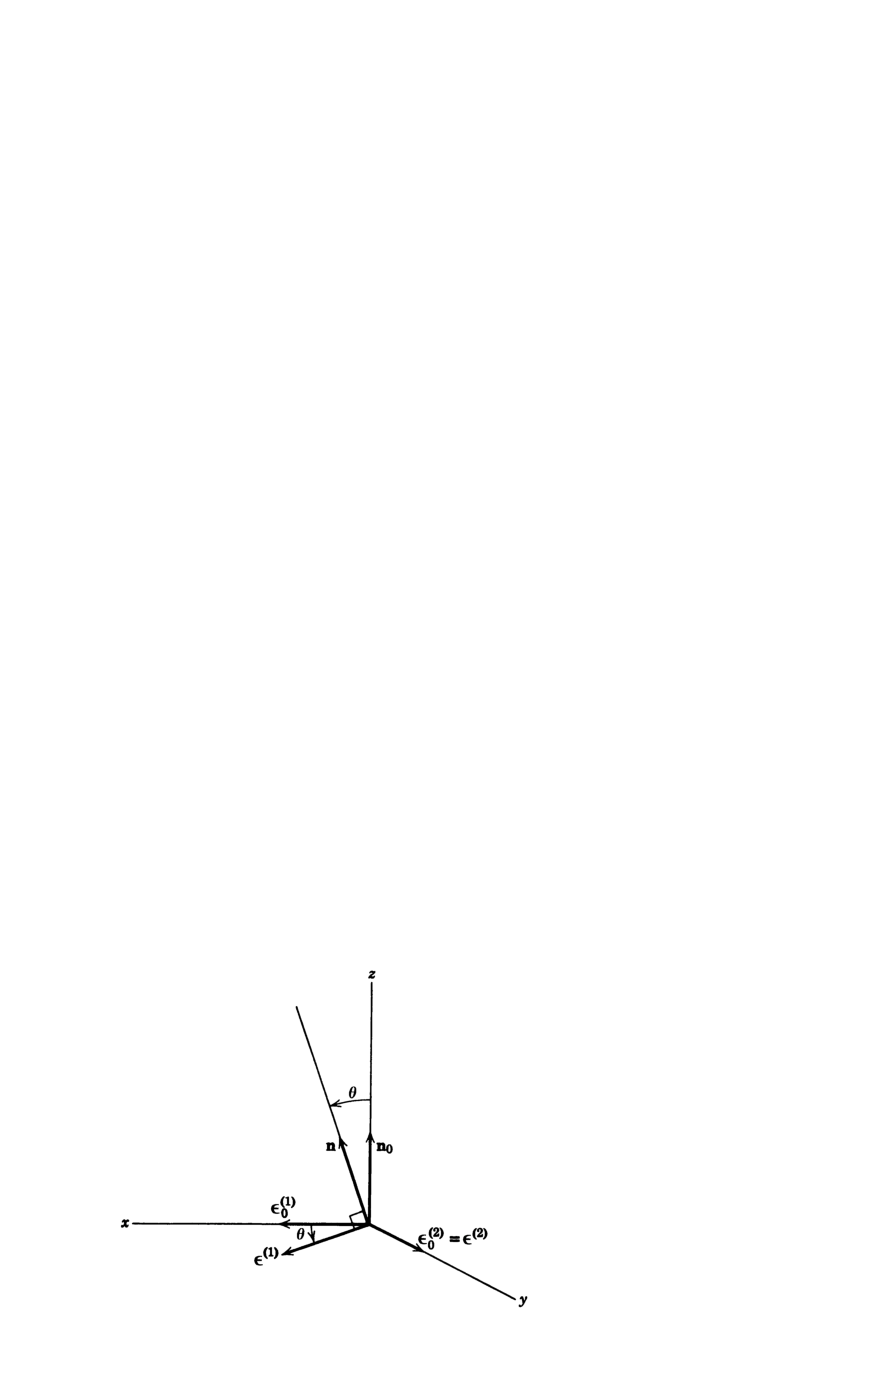
\includegraphics{10-1}
		\caption{(Jackson~{10.1}) Polarization and propagation vectors for the incident and scattered radiation.}
		\label{pol}
	\end{figure}

	The cross section summed over outgoing polarizations is then found by plugging $\veps = \vepsq$ and $\veps = \vepsw$ into Eq.~\refeq{thing2}, and taking the sum.  For the first term,
	\al{
		\dv{\sig}{\Omg} {(\nh, \vepsq; \nho, \vepso)} &= k^4 a^6 \abs{ {\vepsq}^* \vdot \vepso - \frac{1}{2} (\nh \cross {\vepsq}^*) \vdot (\nho \cross \vepso) }^2 \\
		&= k^4 a^6 \abs{ \frac{\nho - (\nh \vdot \nho) \nh}{\sqrt{1 - (\nh \vdot \nho)^2}} \vdot \vepso - \frac{1}{2} \paren{ \nh \cross \frac{\nho - (\nh \vdot \nho) \nh}{\sqrt{1 - (\nh \vdot \nho)^2}} } \vdot (\nho \cross \vepso) }^2 \\
		&= \frac{k^4 a^6}{1 - (\nh \vdot \nho)^2} \abs{ -(\nh \vdot \nho) (\nh \vdot \vepso) - \frac{1}{2} (\nh \cross \nho) \vdot (\nho \cross \vepso) }^2.
	}
	One of the vector identities on the inside cover of Jackson is $(\vaa \cross \vbb) \vdot (\vcc \cross \vdd) = (\vaa \vdot \vcc) (\vbb \vdot \vdd) - (\vaa \vdot \vdd) (\vbb \vdot \vcc)$.  Applying this, we have
	\al{
		\dv{\sig}{\Omg} {(\nh, \vepsq; \nho, \vepso)} &= \frac{k^4 a^6}{1 - (\nh \vdot \nho)^2} \abs{ (\nh \vdot \nho) (\nh \vdot \vepso) + \frac{1}{2} (\nh \vdot \nho) (\nho \vdot \vepso) - \frac{1}{2} (\nh \vdot \vepso) (\nho \vdot \nho) }^2 \\
		&= \frac{k^4 a^6}{1 - (\nh \vdot \nho)^2} \abs{ (\nh \vdot \nho) (\nh \vdot \vepso) - \frac{1}{2} (\nh \vdot \vepso) }^2
		= \frac{k^4 a^6}{1 - (\nh \vdot \nho)^2} \abs{ \nh \vdot \vepso }^2 \brac{ (\nh \vdot \nho) - \frac{1}{2} }^2 \\
		&= \frac{k^4 a^6}{1 - (\nh \vdot \nho)^2} \abs{ \nh \vdot \vepso }^2 \brac{ (\nh \vdot \nho)^2 - (\nh \vdot \nho) + \frac{1}{4} }.
	}
	
	For the second term,
	\al{
		\dv{\sig}{\Omg} {(\nh, \vepsw; \nho, \vepso)} &= k^4 a^6 \abs{ {\vepsw}^* \vdot \vepso - \frac{1}{2} (\nh \cross {\vepsw}^*) \vdot (\nho \cross \vepso) }^2 \\
		&= k^4 a^6 \abs{ \frac{\nh \cross \nho}{\sqrt{1 - (\nh \vdot \nho)^2}} \vdot \vepso - \frac{1}{2} \paren{ \nh \cross \frac{\nh \cross \nho}{\sqrt{1 - (\nh \vdot \nho)^2}} } \vdot (\nho \cross \vepso) }^2 \\
		&= \frac{k^4 a^6}{1 - (\nh \vdot \nho)^2} \abs{ \nh \vdot (\nho \cross \vepso) - \frac{1}{2} [ (\nh \vdot \nho) \nh - (\nh \vdot \nh) \nho ] \vdot (\nho \cross \vepso) }^2 \\
		&= \frac{k^4 a^6}{1 - (\nh \vdot \nho)^2} \abs{ \nh \vdot (\nho \cross \vepso) - \frac{1}{2} [ (\nh \vdot \nho) \nh - \nho ] \vdot (\nho \cross \vepso) }^2 \\
		&= \frac{k^4 a^6}{1 - (\nh \vdot \nho)^2} \abs{ \nh \vdot (\nho \cross \vepso) - \frac{1}{2} (\nh \vdot \nho) \nh \vdot (\nho \cross \vepso) + \frac{1}{2} \epso \vdot (\nho \cross \nho) }^2 \\
		&= \frac{k^4 a^6}{1 - (\nh \vdot \nho)^2} \abs{ \paren{ 1 - \frac{1}{2} (\nh \vdot \nho) } \nh \vdot (\nho \cross \vepso) }^2 \\
		&= \frac{k^4 a^6}{1 - (\nh \vdot \nho)^2} \brac{ 1 - (\nh \vdot \nho) + \frac{1}{4} (\nh \vdot \nho)^2 } \abs{ \nh \vdot (\nho \cross \vepso) }^2.
	}
	
	Summing the two terms, we find
	\aln{
		\dv{\sig}{\Omg} &= \dv{\sig}{\Omg} {(\nh, \vepsq; \nho, \vepso)} + \dv{\sig}{\Omg} {(\nh, \vepsw; \nho, \vepso)} \notag \\
		&= \frac{k^4 a^6}{1 - (\nh \vdot \nho)^2} \curly{ \abs{ \nh \vdot \vepso }^2 \brac{ (\nh \vdot \nho)^2 - (\nh \vdot \nho) + \frac{1}{4} } + \brac{ 1 - (\nh \vdot \nho) + \frac{1}{4} (\nh \vdot \nho)^2 } \abs{ \nh \vdot (\nho \cross \vepso) }^2 } \notag \\
		&= \frac{k^4 a^6}{1 - (\nh \vdot \nho)^2} \bigg\{ \abs{ \nh \vdot \vepso }^2 (\nh \vdot \nho)^2 - \abs{ \nh \vdot \vepso }^2 (\nh \vdot \nho) + \frac{\abs{ \nh \vdot \vepso }^2}{4} + \abs{ \nh \vdot (\nho \cross \vepso) }^2 \notag \\
		&\phantom{mmmmmmmmmmmmmmmmmmmmmmmmmm} - (\nh \vdot \nho) \abs{ \nh \vdot (\nho \cross \vepso) }^2 + \frac{(\nh \vdot \nho)^2 \abs{ \nh \vdot (\nho \cross \vepso) }^2}{4} \bigg\} \notag \\
		&= \frac{k^4 a^6}{1 - (\nh \vdot \nho)^2} \bigg\{ \frac{5 \abs{ \nh \vdot (\nho \cross \vepso) }^2}{4} + \frac{5 \abs{ \nh \vdot \vepso }^2}{4} - (\nh \vdot \nho) \abs{ \nh \vdot (\nho \cross \vepso) }^2 - (\nh \vdot \nho) \abs{ \nh \vdot \vepso }^2 \notag \\
		&\phantom{mmmmmmmmmmmmmmm} - \frac{\abs{ \nh \vdot (\nho \cross \vepso) }^2}{4} - \frac{\abs{ \nh \vdot \vepso }^2}{4} + \frac{(\nh \vdot \nho)^2 \abs{ \nh \vdot (\nho \cross \vepso) }^2}{4} + (\nh \vdot \nho)^2 \abs{ \nh \vdot \vepso }^2 \bigg\} \notag \\
		&= \frac{k^4 a^6}{1 - (\nh \vdot \nho)^2} \curly{ \brac{ \frac{5}{4} - \nh \vdot \nho } \brac{ \abs{ \nh \vdot (\nho \cross \vepso) }^2 + \abs{ \nh \vdot \vepso }^2 } - \brac{ 1 - (\nh \vdot \nho)^2 } \brac{ \frac{\abs{ \nh \vdot (\nho \cross \vepso) }^2}{4} + \abs{ \nh \vdot \vepso }^2 } } \notag \\
		&= \frac{k^4 a^6}{1 - (\nh \vdot \nho)^2} \brac{ \frac{5}{4} - \nh \vdot \nho } \brac{ \abs{ \nh \vdot (\nho \cross \vepso) }^2 + \abs{ \nh \vdot \vepso }^2 } - k^4 a^6 \brac{ \frac{\abs{ \nh \vdot (\nho \cross \vepso) }^2}{4} + \abs{ \nh \vdot \vepso }^2 }. \label{thing2.1}
	}
	
	Since $\nho \vdot \vepso = 0$, we note that
	\eqn{n}{
		\nh = (\nh \vdot \nho) \,\nho + (\nh \vdot \epso) \,\vepso + [ \nh \vdot (\nho \cross \vepso) ] \,(\nho \cross \vepso)
		\qimplies
		1 = (\nh \vdot \nho)^2 + \abs{ \nh \vdot \epso }^2 + \abs{ \nh \vdot (\nho \vdot \vepso) }^2.
	}
	Substituting into Eq.~\refeq{thing2.1},
	\aln{
		\dv{\sig}{\Omg} &= \frac{k^4 a^6}{1 - (\nh \vdot \nho)^2} \brac{ \frac{5}{4} - \nh \vdot \nho } \brac{ 1 - (\nh \vdot \nho)^2 } - k^4 a^6 \brac{ \frac{1}{4} \abs{ \nh \vdot (\nho \cross \vepso) }^2 + \abs{ \nh \vdot \vepso }^2 } \notag \\
		&= \ans{ k^4 a^6 \brac{ \frac{5}{4} - \abs{ \nh \vdot \vepso }^2 - \frac{1}{4} \abs{ \nh \vdot (\nho \cross \vepso) }^2 - \nh \vdot \nho }, } \label{ans2a}
	}
	as we sought to prove. \qed
}

%
%	Jackson 10.1(b)

\prob{}{
	If the incident radiation is linearly polarized, show that the cross section is
	\eq{
		\dv{\sig}{\Omg}(\vepso, \nho, \nh) = k^4 a^6 \brac{ \frac{5}{8} (1 + \cos^2\tht) - \cos\tht - \frac{3}{8} \sin^2\tht \cos(2\phi) },
	}
	where $\nh \vdot \nho = \cos\tht$ and the azimuthal angle $\phi$ is measured from the direction of linear polarization.
}

\sol{
	We choose coordinates as in Fig.~\ref{pol}, such that the direction of linear polarization $\vepso$ points along the $x$ axis and $\nho$ points along the $z$ axis.  Then $\nho \cross \vepso$ points along the $y$ axis.  In spherical coordinates, Eq.~\refeq{n} becomes
	\eqn{n2}{
		\nh = \cos\phi \sin\tht \,\vepso + \sin\phi \sin\tht \,(\nho \cross \vepso) + \cos\tht \,\nho,
	}
	which implies
	\al{
		\cos\phi \sin\tht &= \nh \vdot \epso, &
		\sin\phi \sin\tht &= \nh \vdot (\nho \cross \vepso), &
		\cos\tht &= \nh \vdot \nho.
	}
	Making these substitutions in Eq.~\refeq{ans2a}, we obtain
	\al{
		\dv{\sig}{\Omg} {(\tht, \phi)} &= k^4 a^6 \brac{ \frac{5}{4} - \cos^2 \phi \sin^2 \tht - \frac{1}{4} \sin^2 \phi \sin^2 \tht - \cos\tht } \\
		&= k^4 a^6 \brac{ \frac{5}{4} - \frac{1}{2} [ 1 + \cos(2\phi) ] \sin^2 \tht - \frac{1}{8} [ 1 - \cos(2\phi) ] \sin^2 \tht - \cos\tht } \\
		&= k^4 a^6 \brac{ \frac{5}{4} - \frac{1}{2} (1 - \cos^2 \tht) - \frac{1}{2} \cos(2\phi) \sin^2 \tht - \frac{1}{8} (1 - \cos^2 \tht) + \frac{1}{8} \cos(2\phi) \sin^2 \tht - \cos\tht } \\
		&= \ans{ k^4 a^6 \brac{ \frac{5}{8}(1 + \cos^2 \tht) - \cos\tht - \frac{3}{8} \sin^2 \tht \cos(2\phi) }, }
	}
	where we have used the identities $2 \sin^2\phi = 1 - \cos(2\phi)$, $2 \cos^2\phi = 1 + \cos(2\phi)$, and $\cos^2\tht + \sin^2\tht = 1$. \qed
}

%
%	Jackson 10.1(c)
%

\prob{}{
	What is the ratio of scattered intensities at $\tht = \pi / 2$, $\phi = 0$ and $\tht = \pi / 2$, $\phi = \pi / 2$?  Explain physically in terms of the induced multipoles and their radiation patterns.
}

\sol{
	Firstly, note that
	\al{
		\dv{\sig}{\Omg} {(\pi / 2, 0)} &= k^4 a^6 \brac{ \frac{5}{8} - \frac{3}{8} }
		= \frac{k^4 a^6}{4}, \\
		\dv{\sig}{\Omg} {(\pi / 2, \pi / 2)} &= k^4 a^6 \brac{ \frac{5}{8} + \frac{3}{8} }
		= k^4 a^6,
	}
	so the ratio is
	\eq{
		\ans{ \frac{\dv*{\sig}{\Omg} {(\pi / 2, 0)}}{\dv*{\sig}{\Omg} {(\pi / 2, \pi / 2)}} = \frac{1}{4}. }
	}
		
	According to Jackson~(10.12--13), the electric and magnetic dipole moments of a perfectly conducting sphere are, respectively, 
	\al{
		\vp &= 4\pi \epso a^3 \vEinc, &
		\vm &= 2\pi a^3 \vHinc,
	}
	where $\vEinc$ and $\vHinc$ are the incident fields.  They are given by Jackson~(10.1), wherein
	\al{
		\vEinc &= \vepso E_o e^{i k \nho \vdot \vx}, &
		\vHinc &= \nho \cross \vEinc / \Zo.
	}
	The scattered fields are given by Jackson~(10.2),
	\al{
		\vEsc &= \frac{1}{4\pi \epso} k^2 \frac{e^{i k r}}{r} \brac{ (\nh \cross \vp) \cross \nh - \nh \cross \frac{\vm}{c} }, &
		\vHsc &= \nh \cross \frac{\vEsc}{\Zo}.
	}
	
	When $\phi = 0$, Eq.~\refeq{n2} indicates that $\nh = \vepso$.  Applying the relations above, $\nh$ and $\vp$ therefore point in the same direction.  This means $\nh \cross \vp = \vO$, so $\vEsc$ only has a contribution from the magnetic dipole.  However, When $\phi = \pi / 2$, $\nh = \nho \cross \vepso$ and therefore $\nh$ points in the same direction as $\vm$.  This means $\nh \cross \vm = \vO$, so $\vEsc$ only has a contribution from the electric dipole.  \ans{The ratio $1/4$ indicates that the strength of radiation from a purely electric dipole is four times that from a purely magnetic dipole.}
}